\documentclass[12pt,a4paper]{article}

\usepackage{t1enc}
\usepackage[utf8]{inputenc}
\usepackage[magyar]{babel}
\usepackage{makeidx}
\usepackage{natbib}
\usepackage{hyperref}
\usepackage{enumitem}
\usepackage[version=4]{mhchem}
\usepackage{graphicx}
\usepackage{tabu}
\usepackage{makecell}

\usepackage{amsmath}
\usepackage{amssymb}
\usepackage{amsthm}

\usepackage{tikz}
\usetikzlibrary{positioning}

\author{Gáspár Tamás}
\title{A PageRank és kiszámolása}
\date{}

% számláló és formázás definícióknak: \begin{definicio}
\newcounter{definicioszam}
\newenvironment{definicio}[1]
{{\medskip}\noindent \stepcounter{definicioszam}
{\bfseries{\thedefinicioszam. Definíció: #1\\[1ex]}}}{\bigskip }

%számláló és formázás tételeknek: \begin{tetel}
\newcounter{tszam}
\newenvironment{tetel}[1]
{{\medskip}\noindent \stepcounter{tszam}
{\bfseries{\thetszam. Tétel: #1\\[1ex]}}}{\bigskip }

\begin{document}

%FŐOLDAL ------------------------------------------------------------------

%intézet
\thispagestyle{empty}
\centerline{\textsc{\Large{Szegedi Tudományegyetem}}}
\vspace{0.3 cm}
\centerline{\textsc{\Large{Természettudományi és Informatikai Kar}}}

\vspace*{2 cm}

\centerline{\textsc{\Large{Bolyai Intézet}}}
\vspace{0.3 cm}
\centerline{\textsc{\Large{Sztochasztika tanszék}}}

\vspace{3 cm}

%cím
\centerline{\LARGE{A PageRank és kiszámolása}}
\vspace{0.5 cm}
\centerline{\Large{\textsc{Szakdolgozat}}}

\vspace{3 cm}

%készítő és témavezető táblázat
\begin{center}
	\begin{tabu} to \textwidth { X[l]  X[r] }
		\makecell[l]{Készítette: Gáspár Tamás \\ Matematika BSc hallgató} &
		 \makecell[r]{Témavezető: Dr. Kevei Péter \\ Egyetemi docens \\ Sztochasztika tanszék} \\
	\end{tabu}
\end{center}

\vspace{3 cm}

\centerline{\Large{\textsc{Szeged, 2019}}}

%tartalomjegyzék oldala -------------------------------------------------
\newpage
\thispagestyle{empty}

\tableofcontents

%tényleges kezdet --------------------------------------------------------
\newpage
\setcounter{page}{1}
\fontsize{12}{16}\selectfont

\section{Bevezető}

Dolgozatom témája a PageRank algoritmus, melynek legfőbb alkalmazási területe az internetes weboldalak bizonyos szempontok szerinti rangsorolása.

Ebben a fejezetben röviden ismertetem a PageRank algoritmus történetét és megemlítek egy PageRank számolásához használható, általam készített programot. A második fejezetben a PageRank algoritmus tárgyalásához szükséges alapvető fogalmakat és definíciókat vezetek be. 

\subsection{A PageRank algoritmus története}

A PageRank algoritmust Larry Page és Sergei Brin alkották meg 1998-ban, a Standford Egyetem hallgatóiként. Arra kerestek megoldást, hogy miként lehet az akkoriban robbanásszerű növekedésnek induló internetet weboldalait továbbra is rangsorolni, mivel látszott, hogy az akkor alkalmazott keresőmotorok erre már hamarosan nem lesznek képesek.

Úgy gondolták, hogy a rangsorolás alapja az internet hiperlink struktúrája kell hogy legyen. Feltették, hogy ha egy oldal linkel egy másikra, az kifejezi azt, hogy az oldal készítői megbíznak a linkelt oldalban, ezért az algoritmusukat úgy építették fel, hogy egy oldal fontossága (ezt szintén PageRanknak nevezik) attól függ, hogy mennyi és milyen fontos oldalak linkelnek rá.

Larry Page és Sergei Brin találmánya olyan jól alkalmazhatónak bizonyult, hogy Google néven saját vállalkozást alapítottak. A cég keresőmotorjának alapja máig a PageRank algoritmus, skálázhatóságát mutatja, hogy a Google ma már több mint 130 billió weboldalt indexel. 

\subsection{PageRank program}

Dolgozatomhoz grafikus felhasználói felülettel ellátott asztali alkalmazást is készítettem, Java nyelven. Ez a program képes előre megadott oldalszámú webet különböző paraméterek alapján véletlenszerűen generálni, majd ehhez PageRankot számolni. A 150 oldalnál kisebb méretű webekhez tartozó mátrixokat meg is tudja jeleníteni.

A program és annak forráskódja is letölthető a következő oldalról:

\vspace{0.3 cm}
\textit{https://github.com/Gtomika/PageRank/releases/tag/v4.1}
\vspace{0.3 cm}

 A futtatáshoz a számítógépen telepítve kell hogy legyen a Java.

\section{Alapfogalmak és definíciók}

\subsection{Linkek, web és a lógó oldalak}\label{link_web_logooldal}

Ahhoz hogy PageRankról beszélhessünk, először a web fogalmát kell bevezetni.

\begin{definicio}{Linkhalmaz}
	Legyen V a weboldalak halmaza. Ekkor $L \subset V \times V$ \textbf{linkhalmaz}ban $(v_1,v_2)$ ($v_1, v_2 \in V$ pontosan akkor van benne ha $v_1$ linkel $v_2$-re. 
\end{definicio}

\begin{definicio}{Web}
	Legyen V a weboldalak halmaza, L pedig az ehhez tartozó linkhalmaz. Ekkor a \textbf{web} egy irányított gráf, melynek csúcsai V elemei, élei pedig L elemei, ahol ha $v_1, v_2 \in V$ és $(v_1,v_2) \in L$, akkor az él $v_1$-ből $v_2$-be mutat. 
\end{definicio}

\begin{figure}[h]
	\centering
	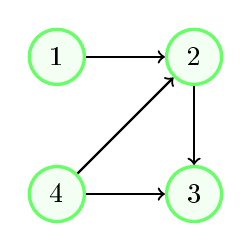
\begin{tikzpicture}[
	roundnode/.style={circle, draw=green!60, fill=green!5, very thick, minimum size=7mm},
	]
	\centering
	%Nodes
	\node[roundnode]      (c1)                     {1};
	\node[roundnode]      (c2)       [right=of c1] {2};
	\node[roundnode]      (c3)       [below=of c2] {3};
	\node[roundnode]      (c4)       [below=of c1] {4};
	
	%Lines
	\draw[->,thick] (c1) -- (c2);
	\draw[->,thick] (c2) -- (c3);
	\draw[->,thick] (c4) -- (c2);
	\draw[->,thick] (c4) -- (c3);
	\end{tikzpicture}
	\caption{Egy 4 oldalból álló web}
\end{figure}

A linkhalmaz definíciója ugyan megengedi azt, hogy egy oldal önmagára linkeljen, mert bár egy valós web esetén ez lehetséges, de a PageRank algoritmus esetén nem akarjuk, hogy az ilyen linkek is beleszámítsanak a rangsorolásba. Ezeket a linkeket ezért egyszerűen elhagyjuk.

Az is megfigyelhető, hogy a definíciókban a linkeknek nincsen multiplicitása, egy oldal vagy linkel egy másikra, vagy nem. Ez azért van, hogy a rangsorolást ne lehessen olyan egyszerűen manipulálni, hogy bizonyos oldalak sok linket tartalmaznak egy másikra.  

Előfordulhat olyan web, ahol bizonyos oldalakról nincsenek kimenő linkek. Az ilyen oldalakat lógó oldalnak nevezzük (azokat a linkeket amelyek rájuk mutatnak pedig lógó linkeknek). A későbbiekben ezek az oldalak problémákat okoznak, ezért megadunk egy módszert, mellyel a ezeket az oldalakat el lehet tüntetni: minden lógó oldalt helyettesítünk egy, az összes másik oldalra linkelővel (ebben a kivételes esetben megengedjük az önmagára linkelést is). 

\bigskip

\begin{minipage}{0.4\textwidth}
	\begin{center}
		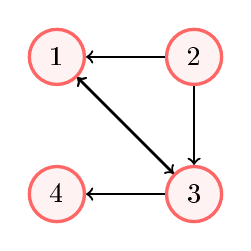
\begin{tikzpicture}[
		roundnode/.style={circle, draw=red!60, fill=red!5, very thick, minimum size=7mm},
		]
		%Nodes
		\node[roundnode]      (c1)                     {1};
		\node[roundnode]      (c2)       [right=of c1] {2};
		\node[roundnode]      (c3)       [below=of c2] {3};
		\node[roundnode]      (c4)       [below=of c1] {4};
		
		%Lines
		\draw[->,thick] (c1) -- (c3);
		\draw[->,thick] (c2) -- (c3);
		\draw[->,thick] (c3) -- (c1);
		\draw[->,thick] (c3) -- (c1);
		\draw[->,thick] (c3) -- (c4);
		\draw[->,thick] (c2) -- (c1);
		\end{tikzpicture}
	\end{center}
\end{minipage}
\begin{minipage}{0.5\textwidth}
	\begin{center}
		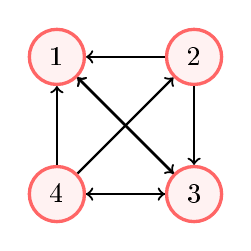
\begin{tikzpicture}[
	roundnode/.style={circle, draw=red!60, fill=red!5, very thick, minimum size=7mm},
	]
	%Nodes
	\node[roundnode]      (c1)                     {1};
	\node[roundnode]      (c2)       [right=of c1] {2};
	\node[roundnode]      (c3)       [below=of c2] {3};
	\node[roundnode]      (c4)       [below=of c1] {4};
	
	%Lines
	\draw[->,thick] (c1) -- (c3);
	\draw[->,thick] (c2) -- (c3);
	\draw[->,thick] (c3) -- (c1);
	\draw[->,thick] (c3) -- (c1);
	\draw[->,thick] (c3) -- (c4);
	\draw[->,thick] (c2) -- (c1);
	\draw[->,thick] (c4) -- (c1);
	\draw[->,thick] (c4) -- (c2);
	\draw[->,thick] (c4) -- (c3);
	\end{tikzpicture}
	\end{center}
\end{minipage}

\bigskip
\centerline{Egy lógó oldallal (4) rendelkező web, és ugyanez a web, helyettesített oldallal.}

\vspace{0.5 cm}

A helyettesítés mögötti heurisztika az, hogy ha egy böngésző egy olyan oldalra érkezik, ahonnan a linkeken keresztül nem tud továbbmenni, akkor véletlenszerűen, egyenletes eloszlás szerint választ az összes oldal közül.

\subsection{A PageRank definíciója}

Egy oldal fontossága azon múlik, hogy mennyi oldal linkel rá, és hogy ezek milyen fontosak. A linkelő oldalak fontosságára azért van szükség, mert enélkül egy oldaltulajdonos tudná úgy növelni a weboldalának fontosságát, hogy rengeteg oldalt hoz létre, melyek mind linkelnek egymásra és a saját oldalára (ezt link farmnak nevezik \cite{lang}).

Egy webet el lehet úgy is képzelni, mint az oldalak demokráciáját ahol minden oldalnak szavazata van és ezt a szavazatot (és még a kapott szavazatokat is) továbbosztja úgy, hogy linkel a többi oldalra.

\begin{definicio}{Weboldal PageRankja}
	Legyen adott egy web, V az oldalak, L a linkek halmaza.
	Legyen $v_i \in V$ oldal PageRankja $r(v_i)$, az oldalról kimenő linkek száma pedig $ |\ v_i |\ $. 
	
	Jelölje $B_i \subset V$ azon oldalak halmazát amelyen linkelnek $v_i$-re, azaz
	\[B_i = \{ v_j \in V: \exists l \in L, \quad l = (v_j,v_i) \} \]
	
	Ekkor bármely $v_i$ oldal PageRankját megkapjuk a következő módon:
	
	\[ r(v_i) = \sum_{v_j \in B_i} \frac{r(v_j)}{ |\ v_j|\ } \]
\end{definicio}

A definícióban megjelenik az is, hogy egy oldalnak mennyi kimenő linkje van. Minél több oldalra linkel, annál kevesebbet fog számítani az ő linkjének értéke. Ez ellensúlyozza a már említett link farmokat.

A szummában szereplő oldalak egyikénél sem lehet a kimenő linkek száma nulla, mert mindegyik oldal eleme a $B_i$ halmaznak, azaz legalább $v_i$-re linkelnek. Előfordulhat, hogy egy oldalra nincs egyetlen link sem. A definícióban ilyenkor egy üres összeg szerepel, azaz az oldal rangja 0.

\bigskip

A PageRank definíciója tehát rekurzív. Egy oldal rangjának meghatározásához minden rá linkelő oldal rangját ismernünk kell. Ha a webünk $n$ db oldalt tartalmaz, akkor a definíció meghatároz $n$ db lineáris egyenletet.

A cél az, hogy olyan algoritmust adjunk meg, amely egyrészt pontosan meghatározza minden oldal PageRankját, másrészt nagyon nagy $n$-re is hatékonyan működik, mind idő-, mind tárigény szempontjából. 

\section{A sajátértékprobléma}

\subsection{Linkmátrix és kapcsolata az egyenletrendszerrel}\label{linkmatrix}

Egy web linkmátrixa az oldalak közötti kapcsolatokat reprezentálja mátrixos formában.

\begin{definicio}{Linkmátrix}
	Legyen adott egy web ahol az oldalak halmaza V. Ennek linkmátrixa legyen $A = (a_{i,j}) \quad i,j = 0,1,...,|\ V |\ $, ahol
	
	\begin{equation}
	a_{i,j}=\begin{cases}
	\frac{1}{ |\ v_i |\ }, & \text{ha $(v_i,v_j) \in L$}.\\
	0, & \text{egyébként}.
	\end{cases}
	\end{equation}
	
\end{definicio}

Tehát a linkmátrix sorai kifejezik azt, hogy egy oldal mennyi és melyik másik oldalakra linkel. Megfigyelhető, hogy amennyiben a web nem tartalmaz lógó oldalt, úgy a linkmátrix sztochasztikus lesz, azaz sorainak összege mindig 1, amennyiben pedig tartalmaz ilyen oldalt, a \ref{link_web_logooldal} alfejezetben megadott helyettesítéssel kapott mátrix már sztochasztikus lesz. 

\bigskip

\begin{minipage}{0.4\textwidth}
	\begin{center}
	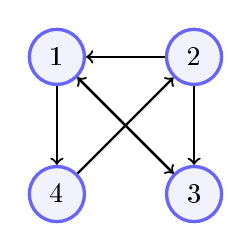
\begin{tikzpicture}[
	roundnode/.style={circle, draw=blue!60, fill=blue!5, very thick, minimum size=7mm},
	]
	%Nodes
	\node[roundnode]      (c1)                     {1};
	\node[roundnode]      (c2)       [right=of c1] {2};
	\node[roundnode]      (c3)       [below=of c2] {3};
	\node[roundnode]      (c4)       [below=of c1] {4};
	
	%Lines
	\draw[->,thick] (c1) -- (c3);
	\draw[->,thick] (c1) -- (c4);
	\draw[->,thick] (c2) -- (c3);
	\draw[->,thick] (c4) -- (c2);
	\draw[->,thick] (c3) -- (c1);
	\draw[->,thick] (c2) -- (c1);
	\end{tikzpicture}
	\end{center}
\end{minipage}
\begin{minipage}{0.5\textwidth}
	\begin{center}
		\[
	  \begin{bmatrix}
	  	0 & 0 & \frac{1}{2} & \frac{1}{2} \\  
	  	\frac{1}{2} & 0 & \frac{1}{2} & 0 \\
	  	1 & 0 & 0 & 0 \\
	    0 & 1 & 0 & 0 \\
	  \end{bmatrix}
	  \]
	\end{center}
\end{minipage}

\bigskip
\centerline{Példa: egy 4 oldalból álló web és linkmátrixa}
\bigskip

Kapcsolat van az oldalak PageRankjának definíciójából kapott egyenletrendszer és a linkmátrix között. Ennek segítségével az egyenletrendszer felírható a következő mátrixegyenletként:

\[ x = x A \]

ahol x az oldalak rangjait tartalmazó vektor. Ezt átalakítva a következőt kapjuk:

\[ x = A^T x \]

Ebből mátrixegyenletből látszik, hogy a keresett vektor az $A^T$ mátrix 1 sajátértékéhez tartozó sajátvektor. Természetesen egy sajátvektor bármilyen nem nulla skalár szorosa is sajátvektor ezért az egyértelműség kedvéért tegyük fel, hogy az általunk keresett vektor az, ahol a komponensek összege 1, ez a későbbiekben hasznos lesz.

\vspace{0.1cm}
\textbf{Megjegyzés:} Ha webnek az internet egy sok oldalból álló részhalmazát választjuk (márpedig a PageRankokat ilyen esetre akarjuk kiszámolni), akkor a linkmátrix nagyon ritka lesz, azaz szinte az összes eleme 0. Ennek oka, hogy az egy oldal által linkelt további oldalak száma elenyésző az összes oldal számához képest. A linkmátrix ritkasága egy számolási szempontból nagyon kedvező tulajdonság. 

\subsection{Az 1 sajátérték}\label{egy_sajatertek}

Felmerül a kérdés, hogy minden $A^T$ mátrixnak sajátértéke-e az 1. Ehhez elég belátni, hogy az $A$ linkmátrixnak az 1 mindig sajátértéke, mivel egy mátrixnak és transzponáltjának a sajátértékei megegyeznek.

\begin{tetel}{Az 1 sajátértéke minden lógó oldalt nem tartalmazó web linkmátrixának}
\end{tetel}
\begin{proof}
	Legyen A egy tetszőleges, lógó oldalt nem tartalmazó, n oldalból álló web linkmátrixa. Ekkor az i. sorhoz $(i = 1,2,...,n)$ tartozó sorösszeg $ |\ v_i |\ \times \frac{1}{|\ v_i |\ } = 1 $, azaz minden ilyen mátrix sztochasztikus.
	
	Legyen e az az n komponensű oszlopvektor, melynek minden komponense 1. Ekkor az
	
	\[ A e = e \] 
	
	egyenlet teljesül, mert az eredményvektor i. komponense $(i = 1,2,...,n)$
	
	\[ \sum_{j=1}^{n}{1 a_{i,j} } = 1 \] 
	
	a mátrix sztochasztikus tulajdonsága miatt. Tehát bármely linkmátrixnak ez az $e$ vektor sajátvektora, 1 sajátértékkel.
	
\end{proof}
\vspace{0.5cm}

Ugyan bármely mátrixnak és transzponáltjának sajátértékei megegyeznek, de az nem igaz, hogy ezen sajátértékekhez tartozó sajátvektorok is azonosak, ezért a fenti tételben bevezetett $e$ vektor nem biztos, hogy megoldása lesz a PageRank definíciója által meghatározott egyenletrendszernek. Ezzel a megoldás egyébként is használhatatlan az oldalak rangsorolásában, mivel minden oldalnak azonos rangot ad.

A lógó oldalakat tartalmazó webek esetén az 1 nem lesz mindig sajátértéke az $A^T$ mátrixnak (lehetnek 0 összegű sorok, ami a fenti bizonyítást elrontja), azonban figyeljük meg, hogy ha elvégezzük a \ref{link_web_logooldal} alfejezetben megadott helyettesítést akkor a kapott mátrix már sztochasztikus lesz, és erre már érvényes az előbbi tétel.

Tehát beláttuk, hogy minden ilyen mátrixnak vagy sajátértéke az 1, vagy egy egyszerű helyettesítéssel el lehet érni, hogy az legyen. 

\subsection{A legnagyobb sajátérték}\label{legnagyobb_sajatertek}

\begin{tetel}{Minden lógó oldalt nem tartalmazó linkmátrix bármely $\lambda$ sajátértékre $ |\ \lambda |\ \leq 1$.}
\end{tetel}

\begin{proof}
	A sajátértékek abszolút értékének felülről becsléséhez alkalmazzuk a Gershgorin körtételt. Eszerint a mátrix összes sajátértékének benne kell lennie legalább egy Gershgorin körben. A Gershgorin körtétel ugyan komplex mátrixokra is érvényes, de a linkmátrix csak valós elemeket tartalmazhat. A köröket meghatározó halmazok: 
	
	\[ K_i = \{ r \in \mathbb{R}: |\ r - a_{i,i} |\ \leq R_i \} \quad i = 1,2,...,n \]
	
	ahol $R_i$ az i. sorösszeg és $a_{i,i}$ az i sorban lévő főátlóbeli elem.
	
	Már korábban beláttuk, hogy a feltételeknek eleget tévő linkmátrixok sztochasztikusak, azaz a sorösszeg minden sornál egy. A linkhalmaz \ref{link_web_logooldal} alfejezetben szereplő definíciójában nem engedjük meg azt, hogy egy oldal önmagára linkeljen, ezért $a_{i,i}$ minden sorra 0.
	
	Ezen állítások miatt a köröket meghatározó halmazok a következőre egyszerűsödnek minden sor esetén:
	
	\[ K_i = \{ r \in \mathbb{R}: |\ r |\ \leq 1 \} \quad i = 1,2,...,n \]
	
	Ebből következik, hogy bármely $\lambda$ sajátértékre $ |\ \lambda |\ \leq 1$-nek teljesülnie kell.
\end{proof}

Beláttuk, hogy az egy minden esetben sajátérték, és azt is hogy ennél (abszolút értékben) nem is lehet nagyobb sajátérték. Ebből azonban nem következik az, hogy domináns is lenne. Előfordulhat olyan eset is, hogy a -1 is sajátérték, vagy az 1 többszörös multiplicitással szerepel.

\subsection{A hatványiteráció}

Ha sok oldalból álló webek esetén akarjuk meghatározni a rangokat, akkor a pontos megoldást adó módszerek nagyon lassúak, ezért közelítő, iteratív módszerre van szükség. Ideális választás a hatványiteráció, mert ebben az esetben elég tárolni mindössze a linkmátrix transzponáltját, és a PageRank vektor éppen aktuális iterációját a számoláshoz.

\vspace{0.2cm}
A hatványiteráció általános alakja:

\[ x^{i+1} = M x^i \]

ahol $M \in \mathbb{R}^{n \times n}$ és $x^0 \in \mathbb{R}^n$.
\vspace{0.2cm}

A hatványiteráció azonban a domináns sajátértékhez tartozó sajátvektorhoz konvergál. Ha ilyen nincsen, akkor nem tudjuk garantálni a konvergenciát. Ahhoz, hogy alkalmazhassuk az 1-hez tartozó sajátvektor megtalálására, vagy be kell látni, hogy az 1 mindig domináns sajátérték, vagy úgy kell módosítani a linkmátrixon, hogy az legyen.

\section{Konvergencia a PageRank vektorhoz}

\subsection{Gondot okozó tényezők}

Amikor egy nagy webhez tartozó PageRank vektort szeretnénk közelíteni, fontos tudni, hogy az iteráció úgy fog viselkedni ahogyan várjuk.

\vspace{0.3cm}
A következő lehetőségeket kell ellenőrizni:

\begin{enumerate}
	\item Biztosan konvergálni fog-e a hatványiteráció?
	\item Ha igen, akkor az indítási helytől függetlenül mindig ugyanabba a vektorba? 
\end{enumerate}

Egyértelmű, hogy az indulási helytől független, biztos konvergenciát a \ref{legnagyobb_sajatertek} alfejezet végén említett szélsőséges esetek ronthatják el \cite{kleinproject}.

Ezek az eseten olyan webek esetén fordulnak elő, amelyek valójában több egymástól független (azaz nincsenek közöttük linkek) webből állnak össze \cite{kurt}.

\vspace{0.3cm}
\begin{minipage}{0.4\textwidth}
	\begin{center}
		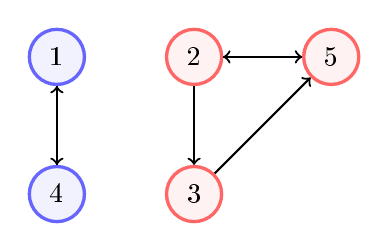
\begin{tikzpicture}[
				broundnode/.style={circle, draw=blue!60, fill=blue!5, very thick, minimum size=7mm},
			rroundnode/.style={circle, draw=red!60, fill=red!5, very thick, minimum size=7mm},
			]
			%Nodes
			\node[broundnode]      (c1)                     {1};
			\node[rroundnode]      (c2)       [right=of c1] {2};
			\node[rroundnode]      (c3)       [below=of c2] {3};
			\node[broundnode]      (c4)       [below=of c1] {4};
			\node[rroundnode]      (c5)       [right=of c2] {5};
			
			%Lines
			\draw[->,thick] (c1) -- (c4);
			\draw[->,thick] (c4) -- (c1);
			\draw[->,thick] (c2) -- (c3);
			\draw[->,thick] (c2) -- (c5);
			\draw[->,thick] (c3) -- (c5);
			\draw[->,thick] (c5) -- (c2);
		\end{tikzpicture}
	\end{center}
\end{minipage}
\begin{minipage}{0.5\textwidth}
	\begin{center}
		\[
		\begin{bmatrix}
		0 & 0 & 0 & 1 & 0 \\
		0 & 0 & \frac{1}{2} & 0 & \frac{1}{2} \\
		0 & 0 & 0 & 0 & 1 \\
		1 & 0 & 0 & 0 & 0 \\
		0 & 1 & 0 & 0 & 0 \\
		\end{bmatrix}
		\]
	\end{center}
\end{minipage}
\vspace{0.3cm}
\newline
\centerline{Két egymással nem érintkező "szubwebből" álló web és linkmátrixa.}
\vspace{0.3cm}

A fenti ábrán látható web linkmátrixának sajátértékei között szerepel a -1 és az 1 is, kétszeres multiplicitással.

\subsection{Webekhez rendelt Markov-láncok}

Vegyünk egy lógó oldalt nem tartalmazó webet. Legyen adott egy úgynevezett véletlen szörföző, aki minden lépésben egyenletes eloszlás szerint választ a jelenlegi oldalon lévő linkek közül és továbbhalad a választott link által mutatott oldalra. A kezdeti eloszlás szintén legyen egyenletes.

Az ehhez a Markov-lánchoz tartozó átmenetmátrix éppen a linkmátrix lesz. A \ref{linkmatrix} alfejezetben meghatároztuk, hogy a keresett PageRank vektor megoldása az $x = xA$ mátrixegyenletnek. Látszik, hogy ez éppen a Markov-lánc invariáns eloszlása. Ezért mondtuk azt, hogy a sajátvektorok közül azt választjuk, ahol a komponensek összege 1.

Ez logikus, hiszen az invariáns eloszlás mutatja, hogy hosszú távon az idő mekkora részét tölti a véletlen szörföző az állapotokban, tehát azok az oldalak lesznek a legfontosabbak, ahol várhatóan a legtöbb időt töltjük.

\vspace{0.1cm}
\textbf{Megjegyzés:} Nem minden webhez rendeletünk egy ilyen Markov-láncot. A lógó oldalakat tartalmazó webek linkmátrixában vannak csupa nulla sorok, melyek elrontják a mátrix sztochasztikusságát, de a \ref{link_web_logooldal} alfejezetben megadott helyettesítéssel kapott webek már megfelelőek. 

\subsection{A konvergencia garantálása}\label{konvergencia_garantalas}

A domináns sajátérték (és ezzel együtt a konvergencia) létezésének garantálásához használjuk fel a Perron–Frobenius tételt.

\vspace{0.1cm}
\textbf{Perron–Frobenius tétel:} Ha egy $A = (a_{i,j})$ $n \times n$ mátrix minden eleme pozitív, akkor biztosan létezik domináns sajátérték, azaz ha a sajátértékek $\lambda_1 , \lambda_2 , ... , \lambda_n$, akkor

\[ \exists r \in \{1,2,...,n\}: \quad \forall i \neq r \quad |\ \lambda_i |\ < \lambda_r  \]

A tétel értelmében tehát az egyértelmű PageRank vektor létezéséhez annyit kell tenni, hogy a linkmátrixot úgy módosítjuk, hogy csak pozitív elemei legyenek.

\begin{definicio}{Google mátrix}
	Legyen $A \in \mathbb{R}^{n \times n}$ egy lógó oldalt nem tartalmazó web linkmátrixa, $S$ pedig egy egy olyan $n \times n$-es mátrix, melynek minden eleme $\frac{1}{n}$. Ekkor a Google mátrix a következőképpen áll elő:
	
	\[ G = \alpha A + (1-\alpha) S \]
	
	ahol $\alpha \in [0,1]$.
\end{definicio}

Látható, hogy a Google mátrix értéke függ az $\alpha$ paramétertől, de majdnem minden esetben (az $\alpha = 1$-et kivéve) a kapott mátrix minden eleme biztosan pozitív, azaz létezik domináns sajátérték és a hatványiteráció indulási helytől függetlenül az ehhez tartozó sajátvektorhoz fog konvergálni.
\vspace{0.1 cm}

\[
\begin{bmatrix}
0 & \frac{1}{2} & \frac{1}{2} & 0 \\
\frac{1}{3} & 0 & \frac{1}{3} & \frac{1}{3} \\
\frac{1}{3} & \frac{1}{3} & 0 & \frac{1}{3} \\
0 & 0 & 1 & 0 \\
\end{bmatrix}, \quad
\begin{bmatrix}
\frac{1}{4} & \frac{1}{4} & \frac{1}{4} & \frac{1}{4} \\
\frac{1}{4} & \frac{1}{4} & \frac{1}{4} & \frac{1}{4} \\
\frac{1}{4} & \frac{1}{4} & \frac{1}{4} & \frac{1}{4} \\
\frac{1}{4} & \frac{1}{4} & \frac{1}{4} & \frac{1}{4} \\
\end{bmatrix}, \quad
\begin{bmatrix}
0,038 & 0,463 & 0,463 & 0,038 \\
0,321 & 0,038 & 0,321 & 0,321 \\
0,321 & 0,321 & 0,38 & 0,321 \\
0,038 & 0,038 & 0,888 & 0,038 \\
\end{bmatrix}
\]

\vspace{0.1 cm}
\centerline{Egy web linkmátrixa, az $S$ mátrix és az $\alpha = 0,7$ paraméterrel kapott Google mátrix.}
\vspace{0.3 cm}

\textbf{Megjegyzés:} A helyettesítés mögötti heurisztika. \newline
Tekintsük a webhez rendelt Markov-láncot. Ezt úgy módosítjuk, hogy a véletlen szörföző most már nem csak a linkeken keresztül juthat el a következő oldalra, hanem bizonyos valószínűséggel egy egyenletes eloszlás szerint választott véletlen oldalra ugrik. Ebben a modellben már nem lehetnek teljesen különálló oldalhalmazok, a véletlen szörföző bárhonnan eljuthat bárhova.

Az így kapott Markov-lánc átmenetmátrixa éppen a Google mátrix lesz, ahol az $\alpha$ paraméter dönt arról, hogy mekkora valószínűséggel követjük a linkeket és mekkorával ugrunk véletlen oldalra.

\section{A Google mátrix és az $\alpha$ paraméter}

\subsection{A Google mátrix tulajdonságai}
%nem ritka, sztochasztikus, stb

A Google mátrix szintén sztochasztikus lesz, bármely $\alpha$ paraméter esetén. A linkmátrixról ($A$) és a csupa $\frac{1}{n}$ komponensből álló ($S$) mátrixokról tudjuk, hogy sztochasztikusak, ezért $\alpha A$ és $(1-\alpha)S$ mátrixok sorösszegei rendre $\alpha$ és $(1-\alpha)$. A Google mátrix esetén így a sorok összege $\alpha+(1-\alpha) = 1$ lesz.

\vspace{0.2cm}

A \ref{linkmatrix} alfejezetben említettük, hogy a linkmátrix általában egy ritka mátrix és hogy ez számítási szempontból nagyon előnyös. A Google mátrix ennek éppen az ellentéte, nemhogy sűrű, de biztosan nem tartalmaz egyetlen 0 elemet sem, ugyanis ez szükséges ha a hatványiteráció konvergenciáját a Perron–Frobenius tétellel akarjuk garantálni. Sűrű mátrixok esetében azonban a mátrixszorzás sokkal lassabb mint ritkáknál.

A Google mátrix sűrűségéből adódó számítási problémát ki lehet küszöbölni. Ha hatványiteráció $i+1$.-ik lépése

\[ x^{i+1} = G x^i \]

ahol $x$ a PageRank vektor, akkor ez ekvivalens a következő alakkal:

\[ x^{i+1} = \alpha A x^i + (1-\alpha)S\] 

Először tehát a linkmátrix skalárszorosával szorozzuk a PageRank vektor jelenlegi iterációját, majd ezután adjuk hozzá a csupa $\frac{1-\alpha}{n}$ elemekből álló mátrixot. Ekkor az elvégzett mátrixszorzásban már nem szerepel a sűrű Google mátrix, de az iteráció eredménye ugyanaz, mitha azzal szoroztunk volna. 

\subsection{Az $\alpha$ paraméter kérdése}

Az előző fejezetben láttuk, hogy szinte bármilyen $\alpha \in [0,1]$ választás esetén (az $\alpha=1$ esetet kivéve) garantáljuk a hatványiteráció konvergenciáját, de felmerül a kérdés, hogy van-e egyéb jelentőség ennek a paraméternek, és ha igen, akkor hogyan válasszuk meg.

A \ref{konvergencia_garantalas} alfejezetben megadott heurisztikából kiderül, hogy $\alpha$ nem lesz más, mint annak a valószínűsége, hogy a véletlen szörföző követi a linkeket, ahelyett, hogy tetszőleges oldalra ugrana. Mivel az oldalak fontosságát a linkek alapján szeretnénk meghatározni (és a PageRankot is így definiáltuk), ezért adódik, hogy $\alpha$-t válasszuk az 1-hez minél közelebbi értéknek, mert így a web struktúrája, a linkek nagy hangsúlyt kapnak a Google mátrixban is. Az 1-hez közeli $\alpha$ azt jelenti, hogy a véletlen szörföző szinte mindig a linkeken keresztül halad tovább.

Tudjuk azonban, hogy a Google, saját PageRank számolásánál $\alpha \approx 0,85$ \cite{lang2} értéket használ. A fentiek ismeretében miért nem 0,9 vagy akár 0,999 ez az érték? 

A válasz az, hogy $\alpha$-tól nagyban függ a konvergencia sebessége, amit a következő fejezetekben indoklunk.

\subsection{A hatványiteráció konvergenciájának sebessége}

Tegyük fel, hogy a mátrixnak, melyre a hatványiterációt szeretnénk alkalmazni a következők a sajátértékei:

\[ |\ \lambda_1 |\ > |\ \lambda_2 |\ \geq |\ \lambda_3 |\ \geq ... \geq |\ \lambda_n |\ \] 

Látható, hogy $\lambda_1$ domináns sajátérték, azaz a hatványiteráció biztosan konvergálni fog. A valódi sajátvektor és az iteráció eredménye közti különbség minden lépésben aszimptotikusan csökken $ |\ \lambda_1 |\ / |\ \lambda_2 |\ $ valamilyen többszörösével \cite{poweriteration}.

$\lambda_1$ domináns sajátérték, ezért a vizsgált hányadosról biztosan tudjuk, hogy:

\[ 1 < |\ \lambda_1 |\ / |\ \lambda_2 |\ \]

Látható, hogy minél kisebb ez a hányados, annál kisebb mértékben fog csökkenni a hiba mértéke az iterációs lépések között, azaz a konvergencia sebessége és a helyzet akkor a legrosszabb amikor

\[ |\ \lambda_1 |\ / |\ \lambda_2 |\ \approx 1 \]

\[ |\ \lambda_1 |\ \approx |\ \lambda_2 |\ \]

A google mátrix estében a sajátértékek

\[ 1 > |\ \lambda_2 |\ \geq |\ \lambda_3 |\ \geq ... \geq |\ \lambda_n |\ \]

ezért a fentebb említett legrosszabb eset a következőképpen módosul:

\[ 1 / |\ \lambda_2 |\ \approx 1 \]

Minél közelebb van tehát a második legnagyobb sajátérték 1-hez (a domináns sajátértékhez), annál lassabb lesz a konvergencia sebessége.

\subsection{$\alpha$ mint sajátérték}

%hivatkozások ---------------------------------------------------------
\bibliography{hivatkozasok}
\bibliographystyle{plain}

\end{document}